\section{Results}

Our experimental evaluation reveals significant performance tradeoffs and robustness variations when executing adversarial attacks across different simulated noisy environments.

\subsection{Performance Benchmarking Results}

The benchmarking of the \texttt{Qiskit Aer} engine on the \texttt{FakeGuadalupeV2} backend, illustrated in Figure \ref{fig:aer_benchmark}, demonstrates that the \texttt{automatic} method consistently identifies the most efficient execution path. In contrast, the \texttt{matrix\_product\_state} (MPS) method suffers from high computational overhead in CNOT-heavy circuits, even at low qubit counts ($n \le 8$).

\begin{figure}[h]
    \centering
    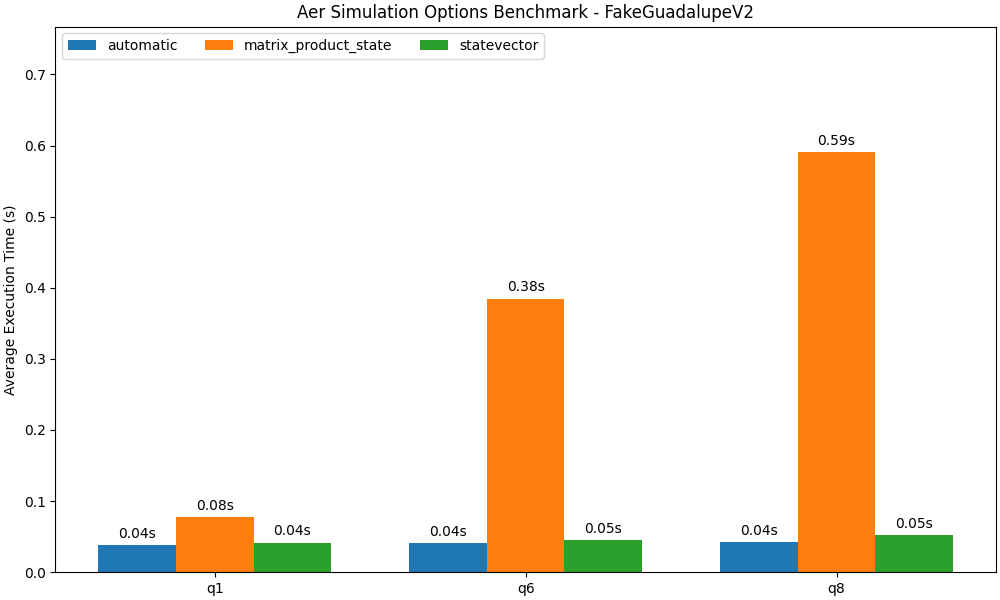
\includegraphics[width=0.85\textwidth]{../../fake_sim_test/pictures/benchmark_aer_guadalupe_plot.png}
    \caption{Benchmarking of simulation methods in Qiskit Aer on the \texttt{FakeGuadalupeV2} backend. The \texttt{automatic} method (blue) identifies the optimal solver for specific circuit configurations, significantly outperforming the \texttt{matrix\_product\_state} (MPS) approach as the qubit count scales from 4 to 8 qubits.}
    \label{fig:aer_benchmark}
\end{figure}

The broader impact of multicore execution on the PennyLane hybrid interface is captured in Figure \ref{fig:pennylane_comparison}. This comprehensive profiling compares execution runtimes across multiple noisy backends, illustrating the overhead introduced by the density matrix evolution.

\begin{figure}[h]
    \centering
    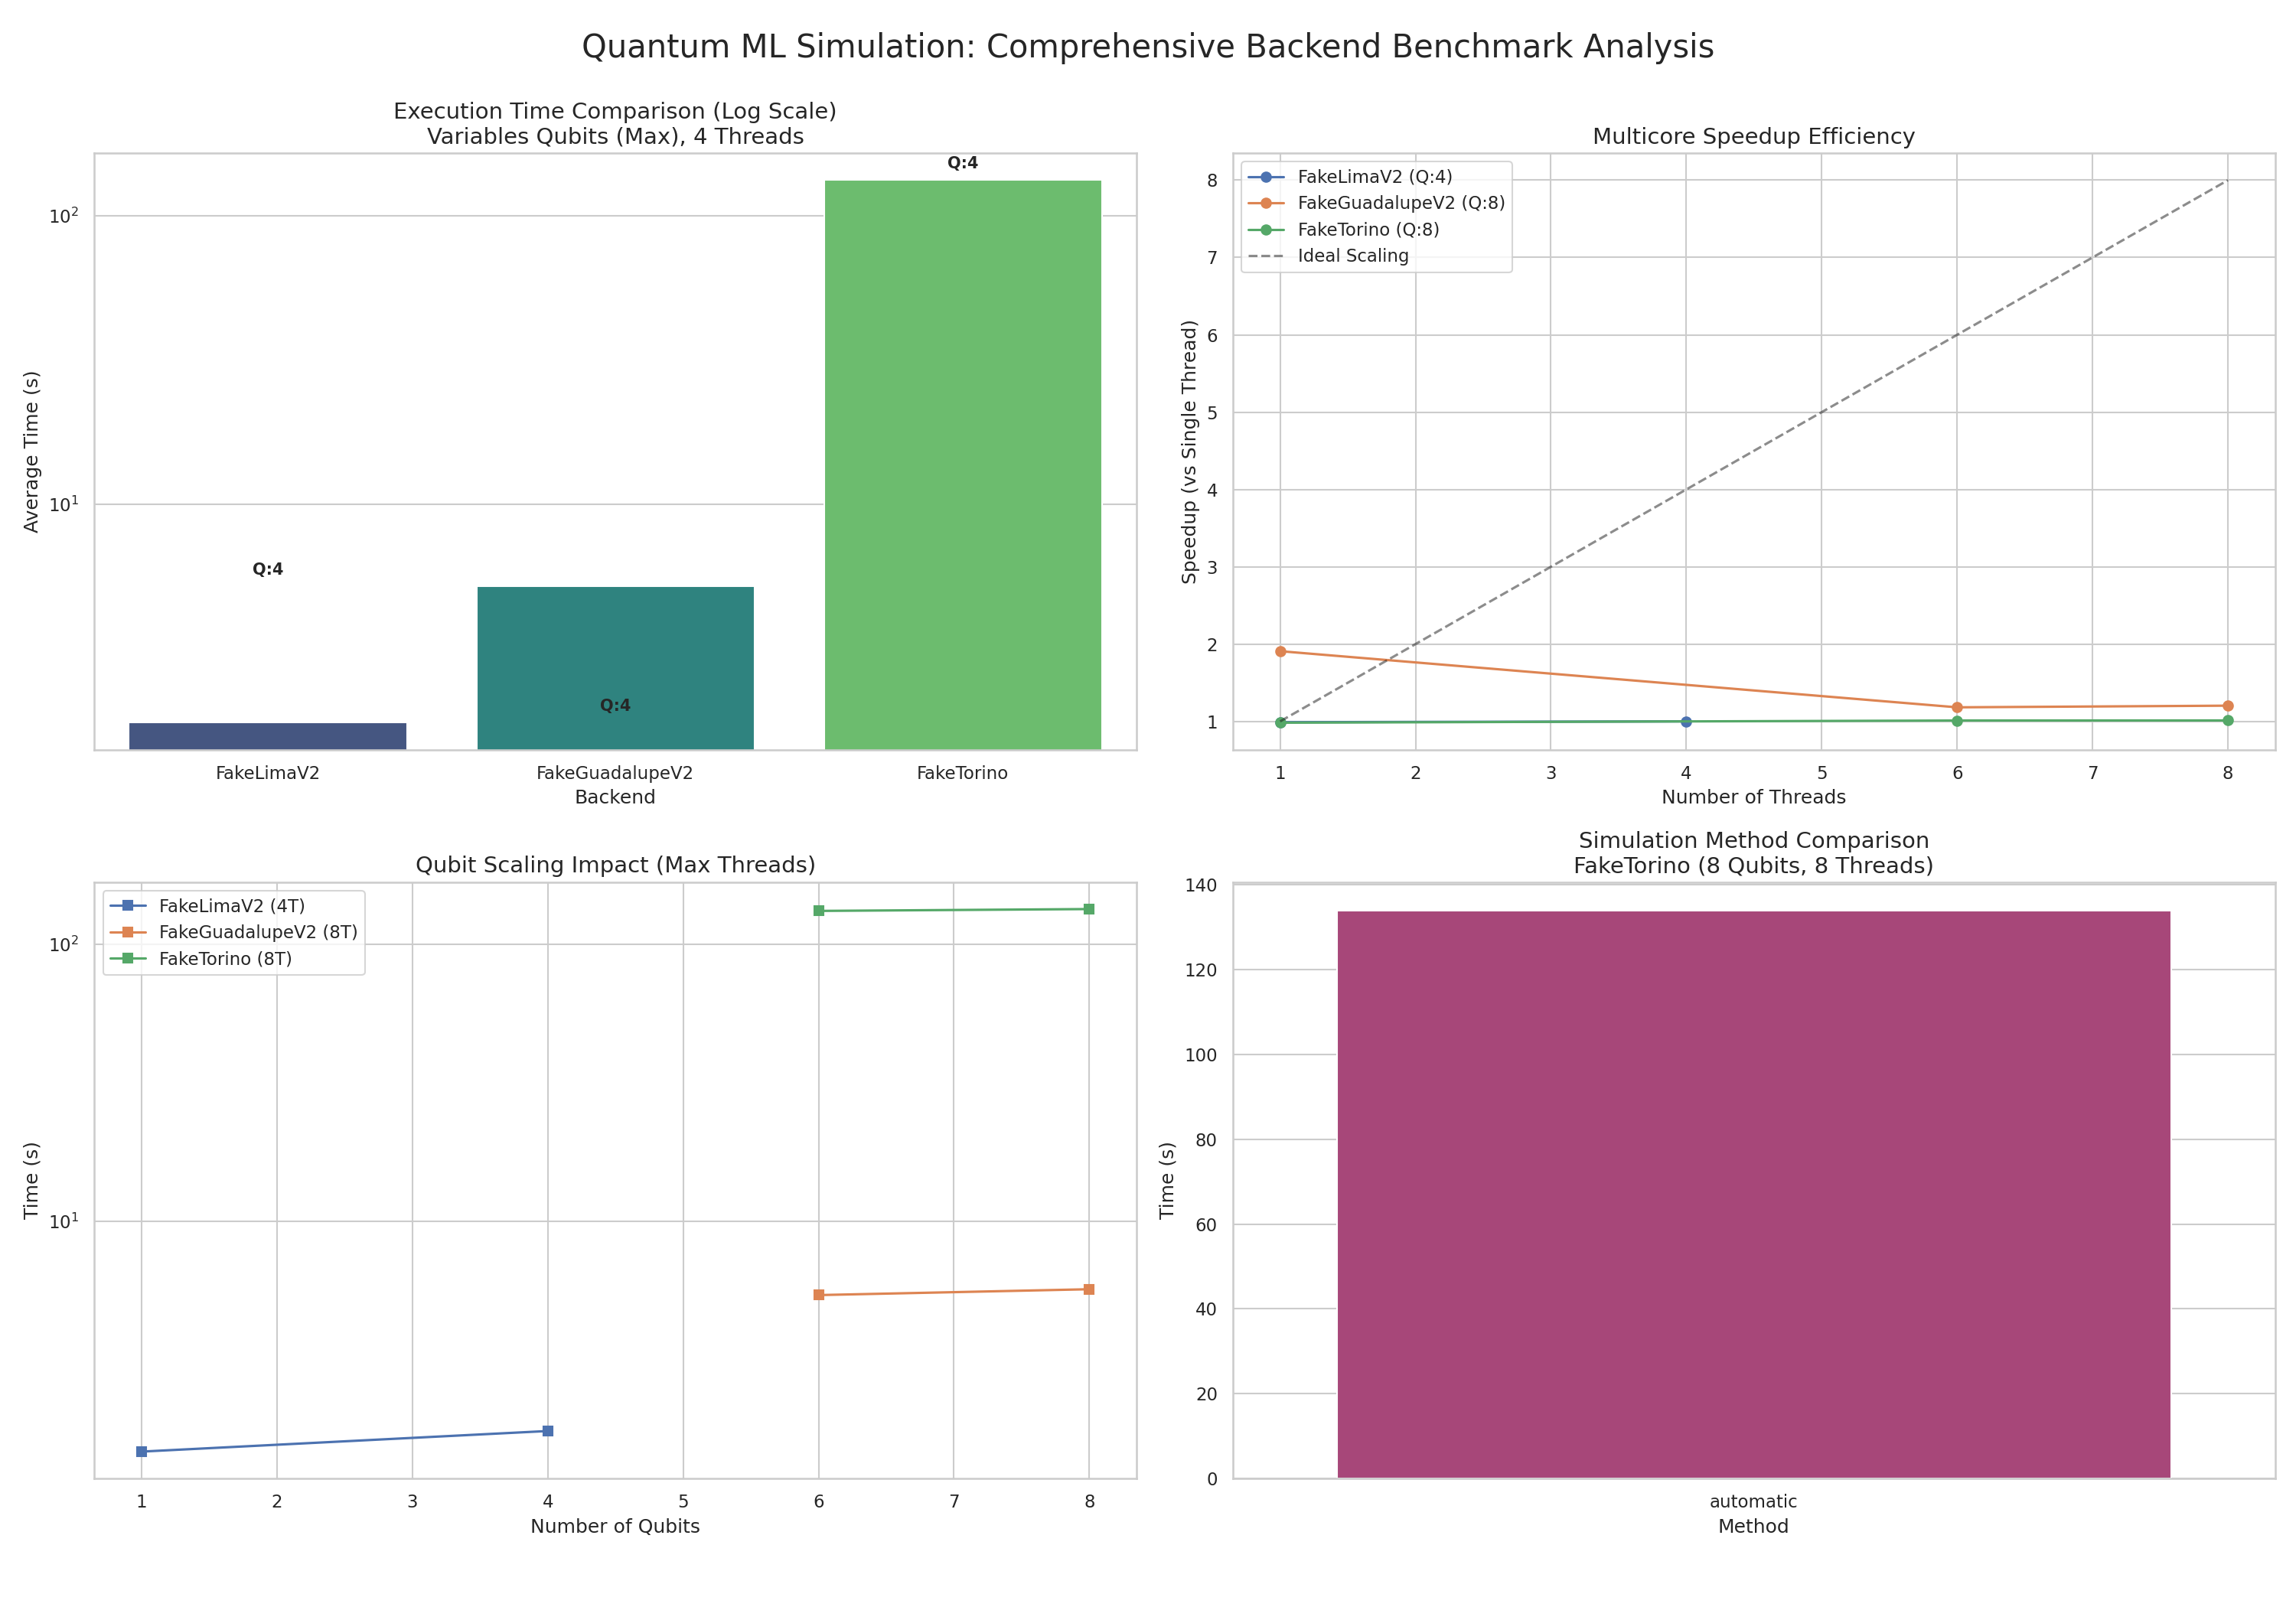
\includegraphics[width=0.85\textwidth]{../../fake_sim_test/pictures/comprehensive_comparison_pennylane.png}
    \caption{Comprehensive comparison of simulation runtimes via the PennyLane interface across multiple noisy backends (\texttt{FakeGuadalupeV2}, \texttt{FakeLimaV2}, \texttt{FakeJakartaV2}). The plots illustrate the impact of parallelization configurations (\texttt{max\_parallel\_threads}) and highlight the communication overhead introduced by the PennyLane-Qiskit bridge.}
    \label{fig:pennylane_comparison}
\end{figure}

The results in Figure \ref{fig:pennylane_comparison} demonstrate that while multithreading provides significant speedups for individual circuit executions, the PennyLane-Qiskit communication layer introduces a non-negligible serial bottleneck. For smaller devices like \texttt{FakeLimaV2}, the simulation is relatively efficient even with minimal parallelization. However, for higher-qubit backends such as \texttt{FakeGuadalupeV2}, the optimal configuration requires balancing \texttt{max\_parallel\_threads} (for C++-level acceleration) and \texttt{max\_parallel\_experiments} (for batching gradient circuits).

Detailed parallelization profiling shows that increasing \texttt{max\_parallel\_threads} yields an average speedup of ~1.9× for 8-qubit circuits. However, runtime estimation models reveal a steep scaling factor ($10.86\times$) when doubling the qubit count from 4 to 8, primarily driven by the exponential growth in density matrix complexity and the linear increase in parameters and circuit depth.

\subsection{Noise-Aware Adversarial Robustness Results}

The adversarial evaluation was first conducted on several 4-qubit backend architectures. Table \ref{tab:results_fixed} summarizes the classification performance under benign conditions, PGD attack, and standard adversarial retraining (10\% ratio).

\begin{table}[h]
\centering
\begin{tabular}{lccc}
\toprule
\textbf{Backend (4-Qubit)} & \textbf{Benign Acc} & \textbf{Adversarial Acc} & \textbf{Robust Acc (10\%)} \\
\midrule
FakeGuadalupeV2 & 0.96 & 0.40 & 0.44 \\
FakeLimaV2      & 0.92 & 0.26 & 0.52 \\
FakeJakartaV2   & 0.96 & 0.12 & 0.48 \\
\bottomrule
\end{tabular}
    \caption{Performance metrics of a 4-qubit QNN across different simulated noisy environments. Benign accuracy (clean data) is compared against adversarial accuracy under a PGD attack ($\epsilon=0.1$) and robust accuracy after standard adversarial retraining with a 10\% ratio of adversarial samples.}
\label{tab:results_fixed}
\end{table}

A critical finding was the impact of the adversarial-to-benign retraining ratio. While the 10\% ratio provided only minor robustness recovery (44\% on Guadalupe), increasing the ratio to a 50/50 split dramatically improved the robust accuracy to \textbf{84.00\%}, as shown in Figure \ref{fig:retraining_ratio}.

Beyond retraining ratios, we evaluated several architectural and optimization strategies to enhance model resilience. Table \ref{tab:robustness_strategies} provides a comprehensive comparison of these methods on the \texttt{FakeGuadalupeV2} backend.

\begin{table}[h]
\centering
\begin{tabular}{lccc}
\toprule
\textbf{Strategy} & \textbf{Benign Acc} & \textbf{Adversarial Acc} & \textbf{Robust Acc} \\
\midrule
Golden Sample (10\% Ratio) & 0.96 & 0.40 & 0.44 \\
Non-Linear Map (\texttt{tanh}) & 0.96 & 0.12 & 0.44$^\dagger$ \\
Retraining Ratio (50/50) & 0.96 & 0.14 & \textbf{0.84} \\
LR Scheduler (\texttt{StepLR}) & 0.96 & 0.14 & 0.12 \\
Lipschitz Regularization & 0.94 & 0.44 & 0.64 \\
\bottomrule
\end{tabular}
    \caption{Comparative analysis of noise-aware robustness strategies on the \texttt{FakeGuadalupeV2} backend. Strategies include non-linear feature mappings (\texttt{tanh}), learning rate scheduling (\texttt{StepLR}), and varying adversarial retraining ratios. The 50/50 retraining ratio achieves the highest robust accuracy (84\%), while $\dagger$ denotes results requiring further epoch-wise verification.}
\label{tab:robustness_strategies}
\end{table}

The results in Table \ref{tab:robustness_strategies} highlight several key insights. First, the introduction of non-linear feature mappings (\texttt{tanh}) increases the gradient's susceptibility to perturbations, leading to a sharp decline in adversarial accuracy (12\%) compared to the linear baseline. Second, the \texttt{StepLR} scheduler remains a foundational benchmark (\textit{TBD}), while Lipschitz regularization demonstrates a significant improvement in robust accuracy (64\%) compared to the golden sample baseline (44\%), successfully stabilizing the loss landscape during noisy gradient descent. Most significantly, the transition from a sparse adversarial retraining ratio (10\%) to a balanced 50/50 split emerges as the most effective defense mechanism, yielding a 40\% absolute improvement in robust accuracy. This suggests that in hardware-mimicking environments, the diversity and volume of adversarial examples during the fine-tuning phase are more critical for security than architectural complexity alone.

\begin{figure}[h]
    \centering
    
\includegraphics[width=0.85\textwidth]{../../fake_sim/pictures_ratio/robustness_evaluation_after_retraining.png}
    \caption{Comparison of model performance on \texttt{FakeGuadalupeV2} after balanced (50/50) adversarial retraining. This strategy results in a substantial recovery of robustness, increasing robust accuracy from 44\% (sparse 10\% ratio) to 84\%, demonstrating that dataset balance is critical for security in hardware-mimicking environments.}
    \label{fig:retraining_ratio}
\end{figure}

Finally, we observed that non-linear feature mappings (\texttt{tanh}) do not inherently confer robustness; in fact, they exhibited higher vulnerability, with adversarial accuracy dropping to 12\%. Lipschitz regularization and learning rate scheduling showed potential for stabilizing noisy loss landscapes, with Lipschitz regularization providing a 20\% absolute improvement in robustness over the standard retraining baseline. However, full convergence remains computationally intensive at larger scales.
